% Options for packages loaded elsewhere
\PassOptionsToPackage{unicode}{hyperref}
\PassOptionsToPackage{hyphens}{url}
%
\documentclass[
  9pt,
]{article}
\usepackage{amsmath,amssymb}
\usepackage{lmodern}
\usepackage{iftex}
\ifPDFTeX
  \usepackage[T1]{fontenc}
  \usepackage[utf8]{inputenc}
  \usepackage{textcomp} % provide euro and other symbols
\else % if luatex or xetex
  \usepackage{unicode-math}
  \defaultfontfeatures{Scale=MatchLowercase}
  \defaultfontfeatures[\rmfamily]{Ligatures=TeX,Scale=1}
\fi
% Use upquote if available, for straight quotes in verbatim environments
\IfFileExists{upquote.sty}{\usepackage{upquote}}{}
\IfFileExists{microtype.sty}{% use microtype if available
  \usepackage[]{microtype}
  \UseMicrotypeSet[protrusion]{basicmath} % disable protrusion for tt fonts
}{}
\makeatletter
\@ifundefined{KOMAClassName}{% if non-KOMA class
  \IfFileExists{parskip.sty}{%
    \usepackage{parskip}
  }{% else
    \setlength{\parindent}{0pt}
    \setlength{\parskip}{6pt plus 2pt minus 1pt}}
}{% if KOMA class
  \KOMAoptions{parskip=half}}
\makeatother
\usepackage{xcolor}
\usepackage[margin=1in]{geometry}
\usepackage{color}
\usepackage{fancyvrb}
\newcommand{\VerbBar}{|}
\newcommand{\VERB}{\Verb[commandchars=\\\{\}]}
\DefineVerbatimEnvironment{Highlighting}{Verbatim}{commandchars=\\\{\}}
% Add ',fontsize=\small' for more characters per line
\usepackage{framed}
\definecolor{shadecolor}{RGB}{248,248,248}
\newenvironment{Shaded}{\begin{snugshade}}{\end{snugshade}}
\newcommand{\AlertTok}[1]{\textcolor[rgb]{0.94,0.16,0.16}{#1}}
\newcommand{\AnnotationTok}[1]{\textcolor[rgb]{0.56,0.35,0.01}{\textbf{\textit{#1}}}}
\newcommand{\AttributeTok}[1]{\textcolor[rgb]{0.77,0.63,0.00}{#1}}
\newcommand{\BaseNTok}[1]{\textcolor[rgb]{0.00,0.00,0.81}{#1}}
\newcommand{\BuiltInTok}[1]{#1}
\newcommand{\CharTok}[1]{\textcolor[rgb]{0.31,0.60,0.02}{#1}}
\newcommand{\CommentTok}[1]{\textcolor[rgb]{0.56,0.35,0.01}{\textit{#1}}}
\newcommand{\CommentVarTok}[1]{\textcolor[rgb]{0.56,0.35,0.01}{\textbf{\textit{#1}}}}
\newcommand{\ConstantTok}[1]{\textcolor[rgb]{0.00,0.00,0.00}{#1}}
\newcommand{\ControlFlowTok}[1]{\textcolor[rgb]{0.13,0.29,0.53}{\textbf{#1}}}
\newcommand{\DataTypeTok}[1]{\textcolor[rgb]{0.13,0.29,0.53}{#1}}
\newcommand{\DecValTok}[1]{\textcolor[rgb]{0.00,0.00,0.81}{#1}}
\newcommand{\DocumentationTok}[1]{\textcolor[rgb]{0.56,0.35,0.01}{\textbf{\textit{#1}}}}
\newcommand{\ErrorTok}[1]{\textcolor[rgb]{0.64,0.00,0.00}{\textbf{#1}}}
\newcommand{\ExtensionTok}[1]{#1}
\newcommand{\FloatTok}[1]{\textcolor[rgb]{0.00,0.00,0.81}{#1}}
\newcommand{\FunctionTok}[1]{\textcolor[rgb]{0.00,0.00,0.00}{#1}}
\newcommand{\ImportTok}[1]{#1}
\newcommand{\InformationTok}[1]{\textcolor[rgb]{0.56,0.35,0.01}{\textbf{\textit{#1}}}}
\newcommand{\KeywordTok}[1]{\textcolor[rgb]{0.13,0.29,0.53}{\textbf{#1}}}
\newcommand{\NormalTok}[1]{#1}
\newcommand{\OperatorTok}[1]{\textcolor[rgb]{0.81,0.36,0.00}{\textbf{#1}}}
\newcommand{\OtherTok}[1]{\textcolor[rgb]{0.56,0.35,0.01}{#1}}
\newcommand{\PreprocessorTok}[1]{\textcolor[rgb]{0.56,0.35,0.01}{\textit{#1}}}
\newcommand{\RegionMarkerTok}[1]{#1}
\newcommand{\SpecialCharTok}[1]{\textcolor[rgb]{0.00,0.00,0.00}{#1}}
\newcommand{\SpecialStringTok}[1]{\textcolor[rgb]{0.31,0.60,0.02}{#1}}
\newcommand{\StringTok}[1]{\textcolor[rgb]{0.31,0.60,0.02}{#1}}
\newcommand{\VariableTok}[1]{\textcolor[rgb]{0.00,0.00,0.00}{#1}}
\newcommand{\VerbatimStringTok}[1]{\textcolor[rgb]{0.31,0.60,0.02}{#1}}
\newcommand{\WarningTok}[1]{\textcolor[rgb]{0.56,0.35,0.01}{\textbf{\textit{#1}}}}
\usepackage{longtable,booktabs,array}
\usepackage{calc} % for calculating minipage widths
% Correct order of tables after \paragraph or \subparagraph
\usepackage{etoolbox}
\makeatletter
\patchcmd\longtable{\par}{\if@noskipsec\mbox{}\fi\par}{}{}
\makeatother
% Allow footnotes in longtable head/foot
\IfFileExists{footnotehyper.sty}{\usepackage{footnotehyper}}{\usepackage{footnote}}
\makesavenoteenv{longtable}
\usepackage{graphicx}
\makeatletter
\def\maxwidth{\ifdim\Gin@nat@width>\linewidth\linewidth\else\Gin@nat@width\fi}
\def\maxheight{\ifdim\Gin@nat@height>\textheight\textheight\else\Gin@nat@height\fi}
\makeatother
% Scale images if necessary, so that they will not overflow the page
% margins by default, and it is still possible to overwrite the defaults
% using explicit options in \includegraphics[width, height, ...]{}
\setkeys{Gin}{width=\maxwidth,height=\maxheight,keepaspectratio}
% Set default figure placement to htbp
\makeatletter
\def\fps@figure{htbp}
\makeatother
\setlength{\emergencystretch}{3em} % prevent overfull lines
\providecommand{\tightlist}{%
  \setlength{\itemsep}{0pt}\setlength{\parskip}{0pt}}
\setcounter{secnumdepth}{-\maxdimen} % remove section numbering
\ifLuaTeX
\usepackage[bidi=basic]{babel}
\else
\usepackage[bidi=default]{babel}
\fi
\babelprovide[main,import]{ngerman}
% get rid of language-specific shorthands (see #6817):
\let\LanguageShortHands\languageshorthands
\def\languageshorthands#1{}
\ifLuaTeX
  \usepackage{selnolig}  % disable illegal ligatures
\fi
\IfFileExists{bookmark.sty}{\usepackage{bookmark}}{\usepackage{hyperref}}
\IfFileExists{xurl.sty}{\usepackage{xurl}}{} % add URL line breaks if available
\urlstyle{same} % disable monospaced font for URLs
\hypersetup{
  pdftitle={Pendel},
  pdfauthor={Milena Mensching Justus Weyers},
  pdflang={de},
  hidelinks,
  pdfcreator={LaTeX via pandoc}}

\title{Pendel}
\author{Milena Mensching Justus Weyers}
\date{2022-12-01}

\begin{document}
\maketitle

\hypertarget{versuch-1}{%
\section{Versuch 1}\label{versuch-1}}

\hypertarget{ziel}{%
\subsection{Ziel}\label{ziel}}

Bestimmung der Erdbeschleunigung \(g\).

\hypertarget{materialien}{%
\subsection{Materialien}\label{materialien}}

\begin{itemize}
\tightlist
\item
  Stativ
\item
  Pendel aus Angelschnur und Metallzylinder
\item
  Maßband
\item
  Messschieber
\item
  Klebeband
\item
  Stoppuhr
\end{itemize}

\hypertarget{versuchsaufbau}{%
\subsection{Versuchsaufbau}\label{versuchsaufbau}}

\begin{itemize}
\tightlist
\item
  Aufstellung des Stativs, Befestigung oberhalb des Tisches
\item
  Befestigung des Maßbandes am Stativ mit Hilfe von Klebeband
\end{itemize}

\begin{figure}
\centering
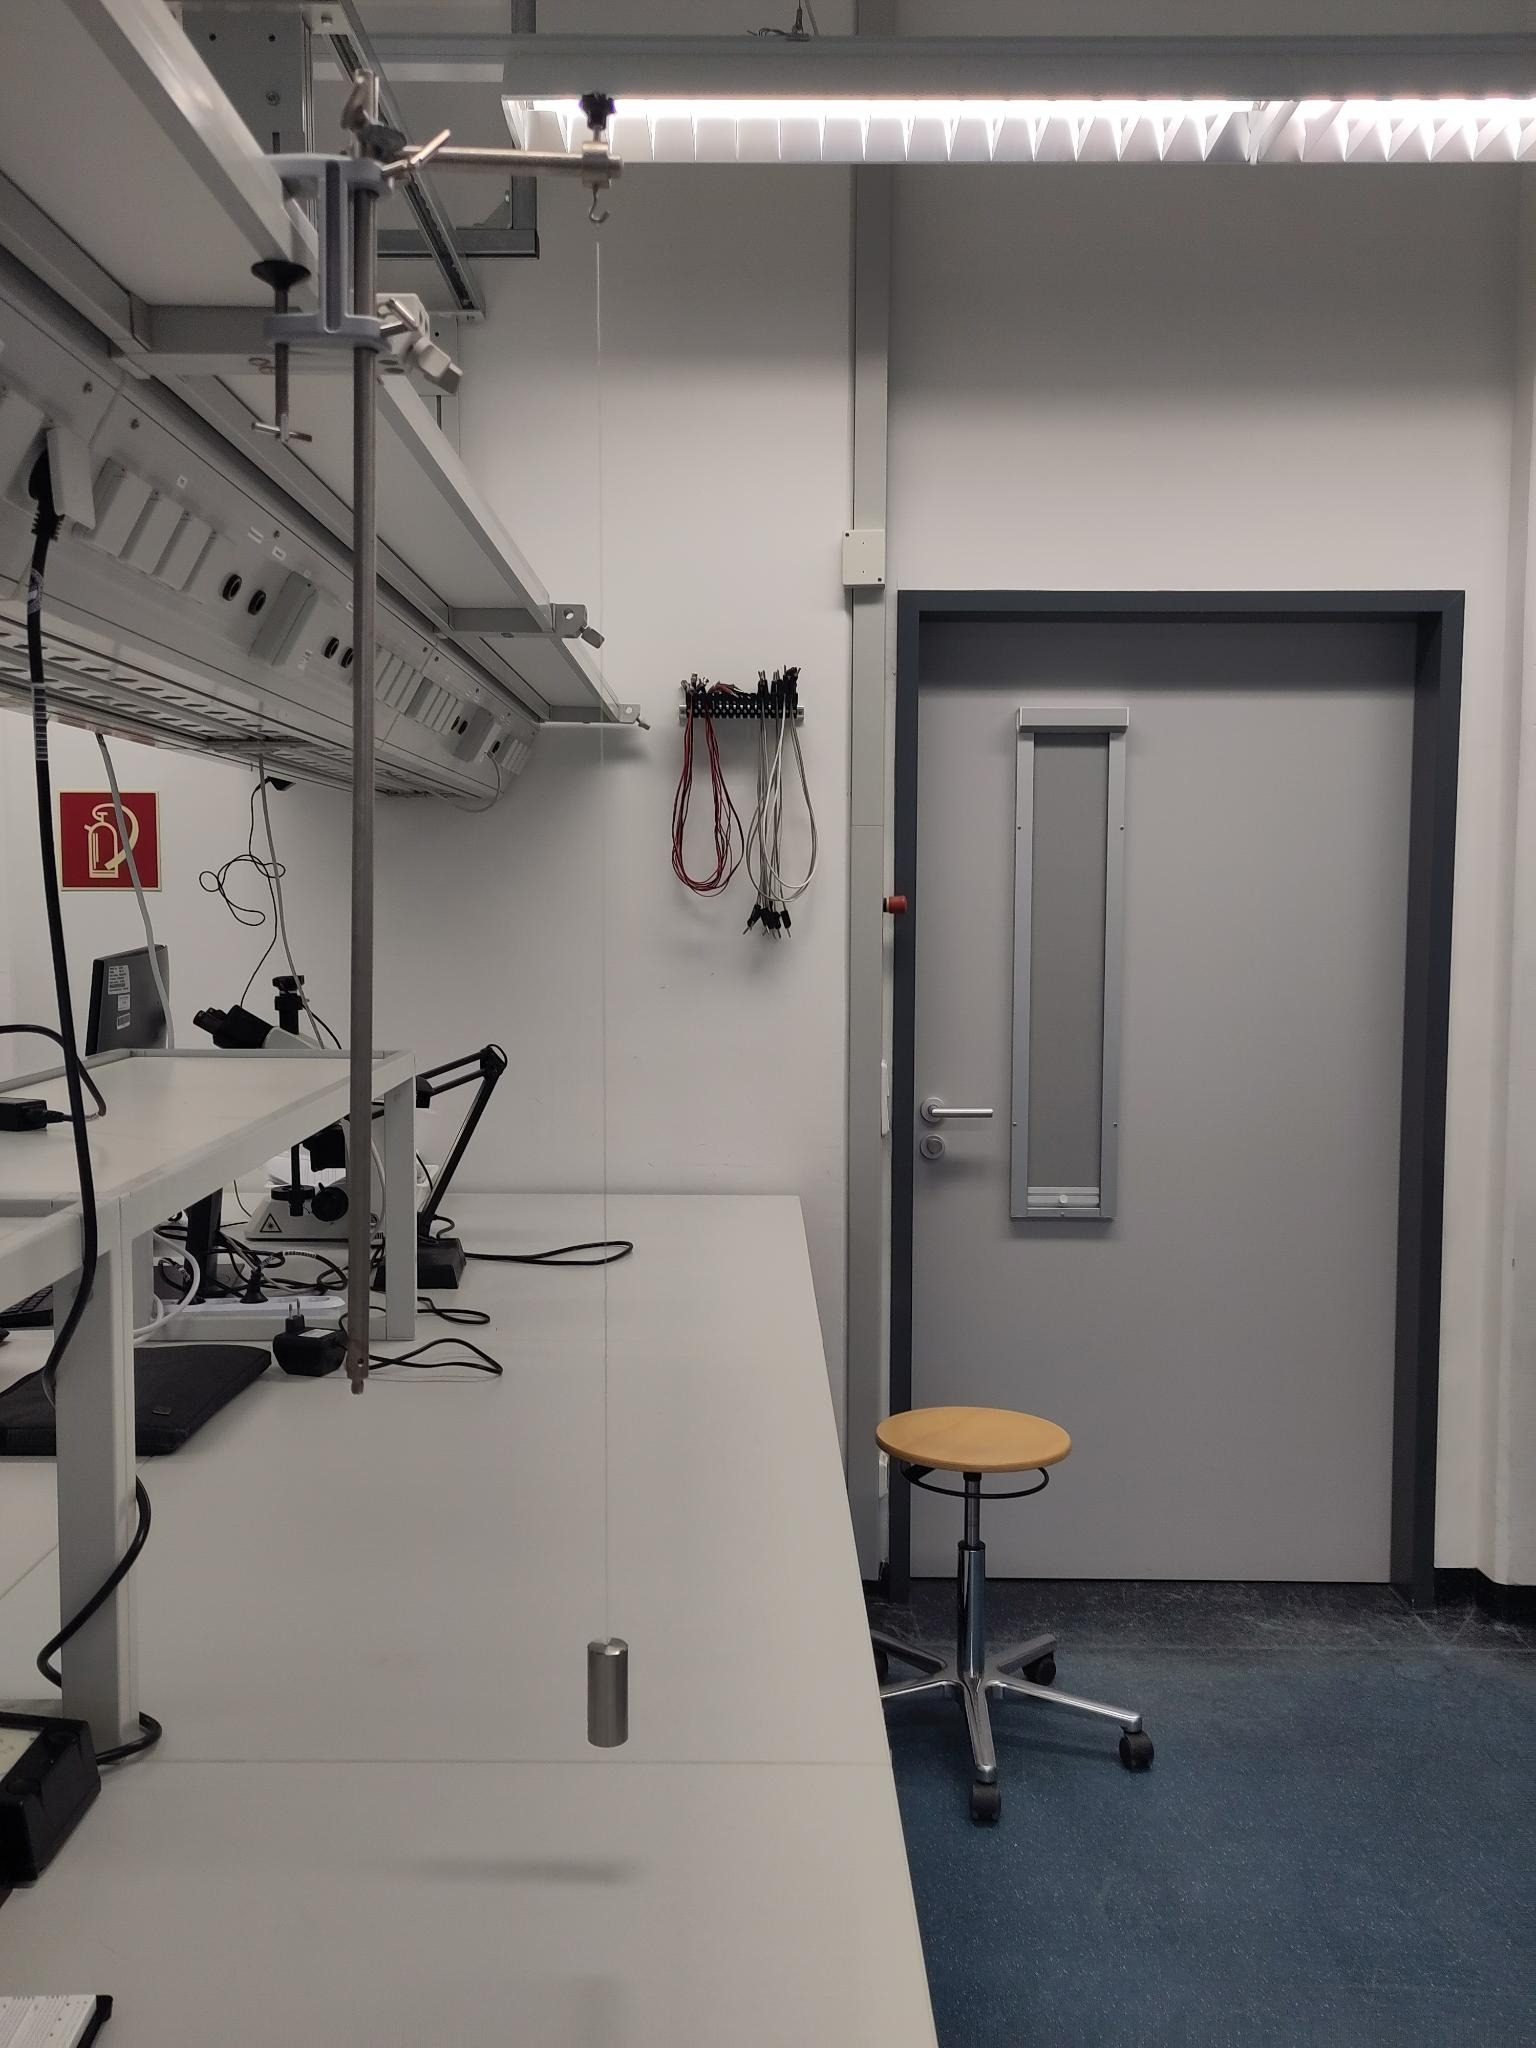
\includegraphics[width=\textwidth,height=0.2\textheight]{Bilder/1.jpeg}
\caption{Versuchsaufbau 1}
\end{figure}

\hypertarget{durchfuxfchrung}{%
\subsection{Durchführung}\label{durchfuxfchrung}}

Nach dem Versuchsaufbau wird mit der Versuchsdurchführung begonnen. Dazu
wird die Pendellänge vermessen, indem am Maßband die Position des
Drehpunktes und die Position der Oberkante des Zylindergewichtes
abgelesen werden. Die Höhe des Zylindergewichtes wird mit einem
Messschieber vermessen.

Im Anschluss wird die Periodendauer für diese Pendellänge bestimmt. Dazu
wird das Pendel aus der Ruheposition ausgelenkt und nach ein paar
Pendelschlägen mit der Zeitmessung begonnen. Die Zeit wird beim
Durchgang durch den Ort der maximalen Geschwindigkeit sowohl gestartet
als auch gestoppt, um die Reaktionszeit möglichst kurz zu halten. Es
werden insgesamt 5 Messungen durchgeführt um einen Mittelwert bilden zu
können.

\hypertarget{fehlerquellen}{%
\subsection{Fehlerquellen}\label{fehlerquellen}}

Beim Auslenken des Pendels gibt es \textbf{unregelmäßige Bewegungen
(Wackeln)}, die entgegen der Pendelbahn laufen.

Beim Abmessen der Pendellänge ist der \textbf{personenbezogene
Ablesefehler} zu erwähnen. Diesen versuchten wir weitestgehend zu
eliminieren, indem nur eine Person eine vollständige Datenreihe aufnahm.

Außerdem verlängert die \textbf{Reaktionszeit} sowohl bei Start als auch
bei Stopp der Messung tendenziell die gemessene Periodendauer. Um diesen
Fehler möglichst gering zu halten, wurden meherere Periodendurchläufe
(10) gemessen und die Periodendauer danach gemittelt. Auch hier nahm nur
eine Person die Datenreihe auf, um die Reaktionszeit ähnlich zu halten.

Folgende Annahmen mussten darüber hinaus getroffen werden:

\begin{itemize}
\tightlist
\item
  Bewegung des Pendelkörpers und des Fadens verläuft reibungsfrei
\item
  Masse des Fadens wird vernachlässigt
\item
  Der Pendelkörper wird nur um eine kleine Strecke ausgelenkt
\item
  Die Angelschnur wird als inelastisch angenommen
\end{itemize}

\hypertarget{messungen}{%
\subsection{Messungen}\label{messungen}}

Im Laufe des Versuches wurden folgende Messwerte aufgenommen, auf die
sich in der folgenden Auswertung bezogen wird:

\begin{longtable}[]{@{}lr@{}}
\caption{Messwerte aus Versuch 1}\tabularnewline
\toprule()
Messgröße & Wert \\
\midrule()
\endfirsthead
\toprule()
Messgröße & Wert \\
\midrule()
\endhead
L1: Position Drehpunkt {[}cm{]} & 4.00 \\
L2: Position Fadenende {[}cm{]} & 88.50 \\
L3: Höhe Zylinder {[}cm{]} & 5.87 \\
10-Periodendauer {[}s{]} & 18.75 \\
10-Periodendauer {[}s{]} & 18.72 \\
10-Periodendauer {[}s{]} & 18.85 \\
10-Periodendauer {[}s{]} & 18.85 \\
10-Periodendauer {[}s{]} & 18.72 \\
\bottomrule()
\end{longtable}

Die fünf Punkte ``10-Periodendauer {[}s{]}'' sind die fünfmal
durchgeführten Messungen, as denen der Mittelwert berechnet werden soll.

\hypertarget{auswertung}{%
\subsection{Auswertung}\label{auswertung}}

\hypertarget{pendelluxe4nge-l-und-unsicherheit-u_l}{%
\subsubsection{\texorpdfstring{Pendellänge L und Unsicherheit
\(u_L\)}{Pendellänge L und Unsicherheit u\_L}}\label{pendelluxe4nge-l-und-unsicherheit-u_l}}

Die Pendellänge \(L\) wird bestimmt, indem Differenz von \(L_1\) und
\(L_2\) berechnet wird, siehe Tabelle im Abschnitt \textit{Messungen}.
Es wird auch darauf geachtet, die Distanz von der Pendeloberkante bis
zum Massenschwerpunkt des Pendels dazuzurechnen. Dafür wird die
Massenverteilung in dem Metallzylinder-Gewicht als homogen angenommen.
Die zu der Fadenlänge zu addierende Länge entspricht dann der halben
Zylinderhöhe \(L_3\). Der Bestwert der errechneten Pendellänge \(L\)
beträgt dann:

\begin{align*}
L&= L_2-L_1+\frac{L_{3}}{2}\\
 &=0,885m-0,04m+\frac{0,0587}{2}m\\
 &=0,87435m.\\
\end{align*}

\begin{Shaded}
\begin{Highlighting}[]
\CommentTok{\# Bestwert Pendellänge in Metern}
\FloatTok{0.885{-}0.04+0.0587}\SpecialCharTok{/}\DecValTok{2}
\end{Highlighting}
\end{Shaded}

\begin{verbatim}
## [1] 0.87435
\end{verbatim}

Die Unsicherheit der Pendellänge setzt sich aus den zu \(L_1\), \(L_2\)
und \(L_3\) gehörigen Messunsicherheiten zusammen: \begin{align*}
u_L&= \sqrt{(\frac{\partial L}{\partial L_2} \cdot u_{Massband})^2+(\frac{\partial L}{\partial L_1} \cdot u_{Massband})^2+(\frac{\partial L}{\partial L_{3}} \cdot u_{Messchieber})^2}\\
&= \sqrt{u_{Massband}^2*(\frac{\partial L}{\partial L_2}^2+\frac{\partial L}{\partial L_1}^2)+(\frac{\partial L}{\partial L_{3}}*u_{Messschieber})^2}\\
&=\sqrt{(\frac{10^{-3}m}{2\sqrt{6}})^2*(1^2+(-1)^2)+(0,5*\frac{10^{-4}m}{2\sqrt{6}})^2}\\
&\approx 0,29 \cdot 10^{-4}m\\
\end{align*} Mit:

\begin{itemize}
  \item Messunsicherheit des Maßbandes: $u_{Massband}=\frac{10^{-3}m}{2\sqrt{6}}$
  \item Messunsicherheit des Messschiebers: $u_{Messschieber}=\frac{10^{-4}m}{2\sqrt{6}}$
\end{itemize}

\begin{Shaded}
\begin{Highlighting}[]
\CommentTok{\# Berechnung von u\_L in R}
\FunctionTok{sqrt}\NormalTok{(}\DecValTok{2}\SpecialCharTok{*}\NormalTok{(((}\DecValTok{10}\SpecialCharTok{**{-}}\DecValTok{3}\NormalTok{)}\SpecialCharTok{/}\NormalTok{(}\DecValTok{2}\SpecialCharTok{*}\FunctionTok{sqrt}\NormalTok{(}\DecValTok{6}\NormalTok{)))}\SpecialCharTok{**}\DecValTok{2}\NormalTok{)}\SpecialCharTok{+}\NormalTok{((}\DecValTok{10}\SpecialCharTok{**{-}}\DecValTok{4}\NormalTok{)}\SpecialCharTok{/}\NormalTok{(}\DecValTok{2}\SpecialCharTok{*}\FunctionTok{sqrt}\NormalTok{(}\DecValTok{6}\NormalTok{)))}\SpecialCharTok{**}\DecValTok{2}\NormalTok{)}
\end{Highlighting}
\end{Shaded}

\begin{verbatim}
## [1] 0.0002893959
\end{verbatim}

Damit beträgt die Pendellänge in diesem Versuch
\(L = (0,87435 \pm 0.00029)m\).

\hypertarget{periodendauer-t-und-unsicherheit-u_t}{%
\subsubsection{\texorpdfstring{Periodendauer T und Unsicherheit
\(u_T\)}{Periodendauer T und Unsicherheit u\_T}}\label{periodendauer-t-und-unsicherheit-u_t}}

Als Zeit für zehn Perioden \(T_{10T}\) in Sekunden wird der Mittelwert
der fünf Messungen aus der Tabelle im Abschnitt \textit{Messungen}
berechnet.

\begin{Shaded}
\begin{Highlighting}[]
\NormalTok{T10 }\OtherTok{\textless{}{-}} \FunctionTok{mean}\NormalTok{(Werte[}\DecValTok{4}\SpecialCharTok{:}\DecValTok{8}\NormalTok{])}
\NormalTok{T10}
\end{Highlighting}
\end{Shaded}

\begin{verbatim}
## [1] 18.778
\end{verbatim}

Die Periodendauer \(T\) in Sekunden wird bestimmt, indem \(T_{10T}\)
durch die Anzahl von Perioden \(n=10\) geteilt wird.

\begin{equation}\label{Pendel:T}
T_{10T} = n*T \Leftrightarrow T = \frac{T_{10T}}{10}
\end{equation}

\begin{Shaded}
\begin{Highlighting}[]
\CommentTok{\# Berechnung der Periodendauer}
\NormalTok{T10}\SpecialCharTok{*}\DecValTok{1}\SpecialCharTok{/}\DecValTok{10}
\end{Highlighting}
\end{Shaded}

\begin{verbatim}
## [1] 1.8778
\end{verbatim}

Die Messunsicherheit der digitalen Stoppuhr \(u_{Stoppuhr}\) ist die
Unsicherheit für \(T_{10T}\). Deren kleinste ablesbare Größenordnung
waren zehn Millisekunden. Damit folgt für \(u_{10T}\):
\(u_{10T}= \frac{a}{2\sqrt{3}} = \frac{0,01s}{2\sqrt{3}} \approx 0,0029s\).

Die Unsicherheit der Periodendauer \(u_T\) ist für zehn Perioden dann
ein Zehntel der Messunsicherheit für zehn Perioden, also
\(u_T=0.00029s\).

Damit ergibt sich die Periodendauer als: \(T=(1.87800 \pm 0.00029)s\).

\hypertarget{ab-hier-noch-weiterarbeiten}{%
\section{Ab hier noch
weiterarbeiten}\label{ab-hier-noch-weiterarbeiten}}

Damit kann der Bestwert der Erdbeschleunigung \(g\) berechnet werden.
Aus \(T=2*\pi*\sqrt{\frac{l}{g}}\) ergibt sich:

\begin{equation*}
\begin{split}
g&=\frac{4*\pi^2*l}{T^2}\\
 &=\frac{4*\pi^2*0,8744m}{(1,878s)^2}\\
 &\approx 9.79 \frac{m}{s^2} 
\end{split}
\end{equation*}

Mit \(l = 0,8744m\)\\
und \(T = 1,878s\)

\begin{Shaded}
\begin{Highlighting}[]
\NormalTok{(}\DecValTok{4}\SpecialCharTok{*}\NormalTok{pi}\SpecialCharTok{**}\DecValTok{2}\SpecialCharTok{*}\FloatTok{0.8744}\NormalTok{)}\SpecialCharTok{/}\NormalTok{(}\FloatTok{1.878}\SpecialCharTok{**}\DecValTok{2}\NormalTok{)}
\end{Highlighting}
\end{Shaded}

\begin{verbatim}
## [1] 9.787656
\end{verbatim}

Messunsicherheit der Erdbeschleunigung \(g\): \begin{equation*}
\begin{split}
u_g&=\sqrt{(\frac{\delta g}{\delta T}*u_T)^2+(\frac{\delta g}{\delta l}*u_l)^2}\\
u_g&=\sqrt{(\frac{-8*\pi^2*l}{T^3}*u_T)^2+(\frac{4*\pi^2}{T^2}*u_l)^2}\\
\\
u_g&\approx \pm ?? \frac{m}{s^2}
\end{split}
\end{equation*}

\hypertarget{interpretation}{%
\subsection{Interpretation}\label{interpretation}}

\hypertarget{versuch-2}{%
\section{Versuch 2}\label{versuch-2}}

Der zweite Versuch läuft analog zum ersten Versuch. Allerdings werden
statt nur einer Messreihe 5 verschiedene - jeweils mit einer anderen
Fadenlänge - gemessen. Um die Pendellängen zu variieren wurde der Faden
für kürzere Fadenlängen mit Klebeband am Zylinder stückchenweise
festgeklebt. Für längere Pendellängen wurden weitere Stücke Angelschnur
an das Pendel geknotet.

\hypertarget{fehlerquellen-1}{%
\subsection{Fehlerquellen}\label{fehlerquellen-1}}

Die Fehlerquellen sind ebenfalls die selben wie beim ersten Versuch.
Allerdings ist hierbei zu bemerken, dass die Reaktioszeit bei kürzeren
Fadenlängen und daraus resultierenden kürzeren Periodendauern
verhältnismäßig zunimmt. Auch von der Bahn abweichende Bewegungen nehmen
bei kürzeren Pendellängen zu. Auch ist nicht unterscuht, wie sich
Klebeband bzw. Knoten im Faden auf das Pendelverhalten auswirken.

\hypertarget{messungen-1}{%
\subsection{Messungen}\label{messungen-1}}

\end{document}
